\documentclass{standalone}
\usepackage{tikz}
\usetikzlibrary{patterns, positioning}

\begin{document}
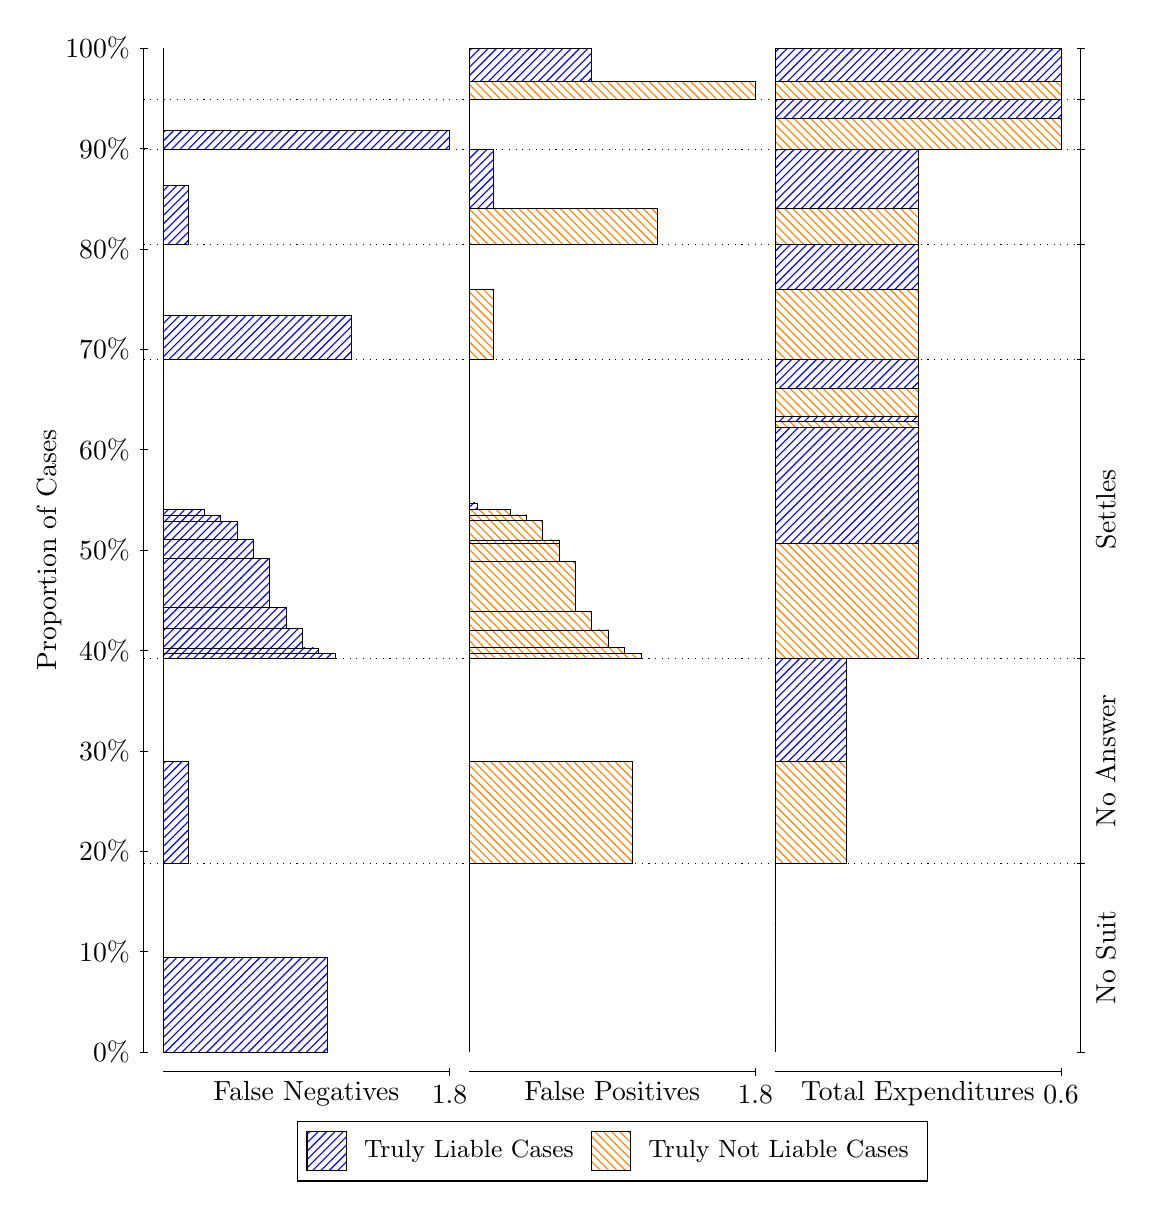
\begin{tikzpicture}
\draw[black, very thin] (1.5,1.75) -- (1.5,14.5);
\node[rotate=90, anchor=center] at (0.3, 8.125) {Proportion of Cases};
\draw[black, very thin] (1.45,1.75) -- (1.55,1.75);
\node[anchor=east] at (1.45, 1.75) {0\%};
\draw[black, very thin] (1.45,3.025) -- (1.55,3.025);
\node[anchor=east] at (1.45, 3.025) {10\%};
\draw[black, very thin] (1.45,4.3) -- (1.55,4.3);
\node[anchor=east] at (1.45, 4.3) {20\%};
\draw[black, very thin] (1.45,5.575) -- (1.55,5.575);
\node[anchor=east] at (1.45, 5.575) {30\%};
\draw[black, very thin] (1.45,6.85) -- (1.55,6.85);
\node[anchor=east] at (1.45, 6.85) {40\%};
\draw[black, very thin] (1.45,8.125) -- (1.55,8.125);
\node[anchor=east] at (1.45, 8.125) {50\%};
\draw[black, very thin] (1.45,9.4) -- (1.55,9.4);
\node[anchor=east] at (1.45, 9.4) {60\%};
\draw[black, very thin] (1.45,10.675) -- (1.55,10.675);
\node[anchor=east] at (1.45, 10.675) {70\%};
\draw[black, very thin] (1.45,11.95) -- (1.55,11.95);
\node[anchor=east] at (1.45, 11.95) {80\%};
\draw[black, very thin] (1.45,13.225) -- (1.55,13.225);
\node[anchor=east] at (1.45, 13.225) {90\%};
\draw[black, very thin] (1.45,14.5) -- (1.55,14.5);
\node[anchor=east] at (1.45, 14.5) {100\%};

\draw[black, very thin] (13.4,1.75) -- (13.4,14.5);
\draw[black, very thin] (13.35,1.75) -- (13.45,1.75);
\node[anchor=west] at (13.35, 1.75) {};
\draw[black, very thin] (13.35,4.1463) -- (13.45,4.1463);
\node[anchor=west] at (13.35, 4.1463) {};
\draw[black, very thin] (13.35,6.7442) -- (13.45,6.7442);
\node[anchor=west] at (13.35, 6.7442) {};
\draw[black, very thin] (13.35,10.541) -- (13.45,10.541);
\node[anchor=west] at (13.35, 10.541) {};
\draw[black, very thin] (13.35,12.007) -- (13.45,12.007);
\node[anchor=west] at (13.35, 12.007) {};
\draw[black, very thin] (13.35,13.216) -- (13.45,13.216);
\node[anchor=west] at (13.35, 13.216) {};
\draw[black, very thin] (13.35,13.85) -- (13.45,13.85);
\node[anchor=west] at (13.35, 13.85) {};
\draw[black, very thin] (13.35,14.5) -- (13.45,14.5);
\node[anchor=west] at (13.35, 14.5) {};

\draw[black, very thin, pattern color=blue, pattern=north east lines] (1.75,1.75) rectangle (3.8262,2.9482);
\draw[black, very thin, pattern color=orange, pattern=north west lines] (1.75,2.9482) rectangle (1.75,4.1463);
\draw[black, very thin, pattern color=blue, pattern=north east lines] (1.75,4.1463) rectangle (2.0614,5.4453);
\draw[black, very thin, pattern color=orange, pattern=north west lines] (1.75,5.4453) rectangle (1.75,6.7442);
\draw[black, very thin, pattern color=blue, pattern=north east lines] (1.75,6.7442) rectangle (3.93,6.8094);
\draw[black, very thin, pattern color=blue, pattern=north east lines] (1.75,6.8094) rectangle (3.7224,6.8806);
\draw[black, very thin, pattern color=blue, pattern=north east lines] (1.75,6.8806) rectangle (3.5148,7.1303);
\draw[black, very thin, pattern color=blue, pattern=north east lines] (1.75,7.1303) rectangle (3.3071,7.3914);
\draw[black, very thin, pattern color=blue, pattern=north east lines] (1.75,7.3914) rectangle (3.0995,8.0163);
\draw[black, very thin, pattern color=blue, pattern=north east lines] (1.75,8.0163) rectangle (2.8919,8.2612);
\draw[black, very thin, pattern color=blue, pattern=north east lines] (1.75,8.2612) rectangle (2.6843,8.4932);
\draw[black, very thin, pattern color=blue, pattern=north east lines] (1.75,8.4932) rectangle (2.4767,8.5626);
\draw[black, very thin, pattern color=blue, pattern=north east lines] (1.75,8.5626) rectangle (2.269,8.6427);
\draw[black, very thin, pattern color=orange, pattern=north west lines] (1.75,8.6427) rectangle (1.75,10.541);
\draw[black, very thin, pattern color=blue, pattern=north east lines] (1.75,10.541) rectangle (4.1376,11.109);
\draw[black, very thin, pattern color=orange, pattern=north west lines] (1.75,11.109) rectangle (1.75,12.007);
\draw[black, very thin, pattern color=blue, pattern=north east lines] (1.75,12.007) rectangle (2.0614,12.76);
\draw[black, very thin, pattern color=orange, pattern=north west lines] (1.75,12.76) rectangle (1.75,13.216);
\draw[black, very thin, pattern color=blue, pattern=north east lines] (1.75,13.216) rectangle (5.3833,13.455);
\draw[black, very thin, pattern color=orange, pattern=north west lines] (1.75,13.455) rectangle (1.75,13.85);
\draw[black, very thin, pattern color=orange, pattern=north west lines] (1.75,13.85) rectangle (1.75,14.08);
\draw[black, very thin, pattern color=blue, pattern=north east lines] (1.75,14.08) rectangle (1.75,14.5);
\draw[black, very thin, pattern color=orange, pattern=north west lines] (5.6333,1.75) rectangle (5.6333,2.9482);
\draw[black, very thin, pattern color=blue, pattern=north east lines] (5.6333,2.9482) rectangle (5.6333,4.1463);
\draw[black, very thin, pattern color=orange, pattern=north west lines] (5.6333,4.1463) rectangle (7.7095,5.4453);
\draw[black, very thin, pattern color=blue, pattern=north east lines] (5.6333,5.4453) rectangle (5.6333,6.7442);
\draw[black, very thin, pattern color=orange, pattern=north west lines] (5.6333,6.7442) rectangle (7.8133,6.8126);
\draw[black, very thin, pattern color=orange, pattern=north west lines] (5.6333,6.8126) rectangle (7.6057,6.8836);
\draw[black, very thin, pattern color=orange, pattern=north west lines] (5.6333,6.8836) rectangle (7.3981,7.1107);
\draw[black, very thin, pattern color=orange, pattern=north west lines] (5.6333,7.1107) rectangle (7.1905,7.3442);
\draw[black, very thin, pattern color=orange, pattern=north west lines] (5.6333,7.3442) rectangle (6.9829,7.983);
\draw[black, very thin, pattern color=orange, pattern=north west lines] (5.6333,7.983) rectangle (6.7752,8.2139);
\draw[black, very thin, pattern color=orange, pattern=north west lines] (5.6333,8.2139) rectangle (6.7752,8.2544);
\draw[black, very thin, pattern color=orange, pattern=north west lines] (5.6333,8.2544) rectangle (6.5676,8.5038);
\draw[black, very thin, pattern color=orange, pattern=north west lines] (5.6333,8.5038) rectangle (6.36,8.5712);
\draw[black, very thin, pattern color=orange, pattern=north west lines] (5.6333,8.5712) rectangle (6.1524,8.6427);
\draw[black, very thin, pattern color=blue, pattern=north east lines] (5.6333,8.6427) rectangle (5.7371,8.7228);
\draw[black, very thin, pattern color=blue, pattern=north east lines] (5.6333,8.7228) rectangle (5.6333,10.541);
\draw[black, very thin, pattern color=orange, pattern=north west lines] (5.6333,10.541) rectangle (5.9448,11.439);
\draw[black, very thin, pattern color=blue, pattern=north east lines] (5.6333,11.439) rectangle (5.6333,12.007);
\draw[black, very thin, pattern color=orange, pattern=north west lines] (5.6333,12.007) rectangle (8.021,12.463);
\draw[black, very thin, pattern color=blue, pattern=north east lines] (5.6333,12.463) rectangle (5.9448,13.216);
\draw[black, very thin, pattern color=orange, pattern=north west lines] (5.6333,13.216) rectangle (5.6333,13.611);
\draw[black, very thin, pattern color=blue, pattern=north east lines] (5.6333,13.611) rectangle (5.6333,13.85);
\draw[black, very thin, pattern color=orange, pattern=north west lines] (5.6333,13.85) rectangle (9.2667,14.08);
\draw[black, very thin, pattern color=blue, pattern=north east lines] (5.6333,14.08) rectangle (7.1905,14.5);
\draw[black, very thin, pattern color=orange, pattern=north west lines] (9.5167,1.75) rectangle (9.5167,2.9482);
\draw[black, very thin, pattern color=blue, pattern=north east lines] (9.5167,2.9482) rectangle (9.5167,4.1463);
\draw[black, very thin, pattern color=orange, pattern=north west lines] (9.5167,4.1463) rectangle (10.425,5.4453);
\draw[black, very thin, pattern color=blue, pattern=north east lines] (9.5167,5.4453) rectangle (10.425,6.7442);
\draw[black, very thin, pattern color=orange, pattern=north west lines] (9.5167,6.7442) rectangle (11.333,8.2139);
\draw[black, very thin, pattern color=blue, pattern=north east lines] (9.5167,8.2139) rectangle (11.333,9.6838);
\draw[black, very thin, pattern color=orange, pattern=north west lines] (9.5167,9.6838) rectangle (11.333,9.7553);
\draw[black, very thin, pattern color=blue, pattern=north east lines] (9.5167,9.7553) rectangle (11.333,9.8204);
\draw[black, very thin, pattern color=orange, pattern=north west lines] (9.5167,9.8204) rectangle (11.333,10.178);
\draw[black, very thin, pattern color=blue, pattern=north east lines] (9.5167,10.178) rectangle (11.333,10.541);
\draw[black, very thin, pattern color=orange, pattern=north west lines] (9.5167,10.541) rectangle (11.333,11.439);
\draw[black, very thin, pattern color=blue, pattern=north east lines] (9.5167,11.439) rectangle (11.333,12.007);
\draw[black, very thin, pattern color=orange, pattern=north west lines] (9.5167,12.007) rectangle (11.333,12.463);
\draw[black, very thin, pattern color=blue, pattern=north east lines] (9.5167,12.463) rectangle (11.333,13.216);
\draw[black, very thin, pattern color=orange, pattern=north west lines] (9.5167,13.216) rectangle (13.15,13.611);
\draw[black, very thin, pattern color=blue, pattern=north east lines] (9.5167,13.611) rectangle (13.15,13.85);
\draw[black, very thin, pattern color=orange, pattern=north west lines] (9.5167,13.85) rectangle (13.15,14.08);
\draw[black, very thin, pattern color=blue, pattern=north east lines] (9.5167,14.08) rectangle (13.15,14.5);
\draw[black, dotted] (1.5,4.1463) -- (13.4,4.1463);
\draw[black, dotted] (1.5,6.7442) -- (13.4,6.7442);
\draw[black, dotted] (1.5,10.541) -- (13.4,10.541);
\draw[black, dotted] (1.5,12.007) -- (13.4,12.007);
\draw[black, dotted] (1.5,13.216) -- (13.4,13.216);
\draw[black, dotted] (1.5,13.85) -- (13.4,13.85);
\draw[black, very thin] (1.75,1.5) -- (5.3833,1.5);
\node[anchor=north] at (3.5667, 1.5) {False Negatives};
\draw[black, very thin] (5.3833,1.45) -- (5.3833,1.55);
\node[anchor=north] at (5.3833, 1.45) {1.8};

\draw[black, very thin] (5.6333,1.5) -- (9.2667,1.5);
\node[anchor=north] at (7.45, 1.5) {False Positives};
\draw[black, very thin] (9.2667,1.45) -- (9.2667,1.55);
\node[anchor=north] at (9.2667, 1.45) {1.8};

\draw[black, very thin] (9.5167,1.5) -- (13.15,1.5);
\node[anchor=north] at (11.333, 1.5) {Total Expenditures};
\draw[black, very thin] (13.15,1.45) -- (13.15,1.55);
\node[anchor=north] at (13.15, 1.45) {0.6};

\node[black, centered, rotate=90] at (13.72, 2.9482) {No Suit};
\node[black, centered, rotate=90] at (13.72, 5.4453) {No Answer};
\node[black, centered, rotate=90] at (13.72, 8.6427) {Settles};





\draw (7.449999999999999,1.5) node[draw=none] (baseCoordinate) {};
\begin{scope}[align=center]
        \matrix[scale=0.5, draw=black, below=0.5cm of baseCoordinate, nodes={draw}, column sep=0.1cm]{
            \node[rectangle, draw, minimum width=0.5cm, minimum height=0.5cm, pattern=north east lines, pattern color=blue] {}; &
            \node[draw=none, font=\small] (B) {Truly Liable Cases}; &
            \node[rectangle, draw, minimum width=0.5cm, minimum height=0.5cm, pattern=north west lines, pattern color=orange] {}; &
            \node[draw=none, font=\small] (B) {Truly Not Liable Cases}; \\
            };
\end{scope}

\end{tikzpicture}
\end{document}